% Created by tikzDevice version 0.8.1 on 2015-05-29 13:30:03
% !TEX encoding = UTF-8 Unicode
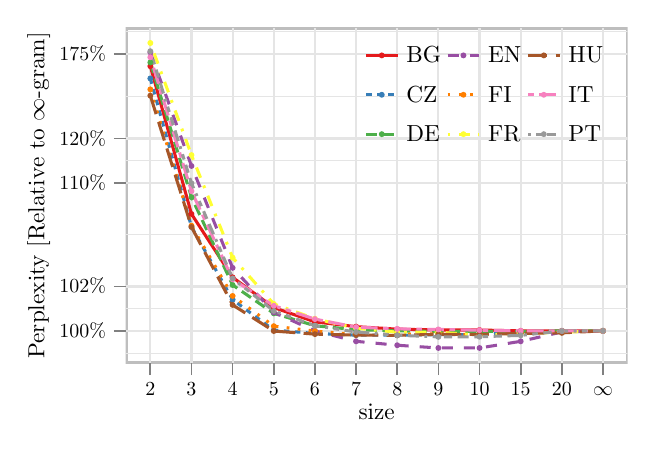
\begin{tikzpicture}[x=1pt,y=1pt]
\definecolor{fillColor}{RGB}{255,255,255}
\path[use as bounding box,fill=fillColor,fill opacity=0.00] (0,0) rectangle (216.81,144.54);
\begin{scope}
\path[clip] (  0.00,  0.00) rectangle (216.81,144.54);
\definecolor{fillColor}{RGB}{255,255,255}

\path[fill=fillColor] (  0.00,  0.00) rectangle (216.81,144.54);
\end{scope}
\begin{scope}
\path[clip] ( 35.40, 23.29) rectangle (216.81,144.54);
\definecolor{drawColor}{RGB}{190,190,190}

\path[draw=drawColor,line width= 1.5pt,line join=round,line cap=round] ( 35.40, 23.29) rectangle (216.81,144.54);
\definecolor{drawColor}{gray}{0.90}

\path[draw=drawColor,line width= 0.3pt,line join=round] ( 35.40, 26.94) --
	(216.81, 26.94);

\path[draw=drawColor,line width= 0.3pt,line join=round] ( 35.40, 43.01) --
	(216.81, 43.01);

\path[draw=drawColor,line width= 0.3pt,line join=round] ( 35.40, 69.72) --
	(216.81, 69.72);

\path[draw=drawColor,line width= 0.3pt,line join=round] ( 35.40, 96.43) --
	(216.81, 96.43);

\path[draw=drawColor,line width= 0.3pt,line join=round] ( 35.40,119.79) --
	(216.81,119.79);

\path[draw=drawColor,line width= 0.3pt,line join=round] ( 35.40,143.16) --
	(216.81,143.16);

\path[draw=drawColor,line width= 0.8pt,line join=round] ( 35.40, 34.98) --
	(216.81, 34.98);

\path[draw=drawColor,line width= 0.8pt,line join=round] ( 35.40, 51.05) --
	(216.81, 51.05);

\path[draw=drawColor,line width= 0.8pt,line join=round] ( 35.40, 88.39) --
	(216.81, 88.39);

\path[draw=drawColor,line width= 0.8pt,line join=round] ( 35.40,104.46) --
	(216.81,104.46);

\path[draw=drawColor,line width= 0.8pt,line join=round] ( 35.40,135.12) --
	(216.81,135.12);

\path[draw=drawColor,line width= 0.8pt,line join=round] ( 44.32, 23.29) --
	( 44.32,144.54);

\path[draw=drawColor,line width= 0.8pt,line join=round] ( 59.19, 23.29) --
	( 59.19,144.54);

\path[draw=drawColor,line width= 0.8pt,line join=round] ( 74.06, 23.29) --
	( 74.06,144.54);

\path[draw=drawColor,line width= 0.8pt,line join=round] ( 88.93, 23.29) --
	( 88.93,144.54);

\path[draw=drawColor,line width= 0.8pt,line join=round] (103.80, 23.29) --
	(103.80,144.54);

\path[draw=drawColor,line width= 0.8pt,line join=round] (118.67, 23.29) --
	(118.67,144.54);

\path[draw=drawColor,line width= 0.8pt,line join=round] (133.54, 23.29) --
	(133.54,144.54);

\path[draw=drawColor,line width= 0.8pt,line join=round] (148.41, 23.29) --
	(148.41,144.54);

\path[draw=drawColor,line width= 0.8pt,line join=round] (163.28, 23.29) --
	(163.28,144.54);

\path[draw=drawColor,line width= 0.8pt,line join=round] (178.15, 23.29) --
	(178.15,144.54);

\path[draw=drawColor,line width= 0.8pt,line join=round] (193.02, 23.29) --
	(193.02,144.54);

\path[draw=drawColor,line width= 0.8pt,line join=round] (207.89, 23.29) --
	(207.89,144.54);
\definecolor{drawColor}{RGB}{228,26,28}

\path[draw=drawColor,line width= 1.1pt,line join=round] ( 44.32,130.63) --
	( 59.19, 77.21) --
	( 74.06, 54.31) --
	( 88.93, 43.41) --
	(103.80, 38.23) --
	(118.67, 36.51) --
	(133.54, 35.60) --
	(148.41, 35.29) --
	(163.28, 35.29) --
	(178.15, 34.98) --
	(193.02, 34.98) --
	(207.89, 34.98);
\definecolor{drawColor}{RGB}{55,126,184}

\path[draw=drawColor,line width= 1.1pt,dash pattern=on 2pt off 2pt ,line join=round] ( 44.32,126.19) --
	( 59.19, 72.56) --
	( 74.06, 46.26) --
	( 88.93, 35.27) --
	(103.80, 34.06) --
	(118.67, 33.43) --
	(133.54, 33.43) --
	(148.41, 33.59) --
	(163.28, 33.59) --
	(178.15, 34.67) --
	(193.02, 34.82) --
	(207.89, 34.98);
\definecolor{drawColor}{RGB}{77,175,74}

\path[draw=drawColor,line width= 1.1pt,dash pattern=on 4pt off 2pt ,line join=round] ( 44.32,131.98) --
	( 59.19, 83.27) --
	( 74.06, 51.55) --
	( 88.93, 41.31) --
	(103.80, 36.83) --
	(118.67, 35.40) --
	(133.54, 34.98) --
	(148.41, 34.76) --
	(163.28, 34.76) --
	(178.15, 34.76) --
	(193.02, 34.98) --
	(207.89, 34.98);
\definecolor{drawColor}{RGB}{152,78,163}

\path[draw=drawColor,line width= 1.1pt,dash pattern=on 4pt off 4pt ,line join=round] ( 44.32,135.63) --
	( 59.19, 94.56) --
	( 74.06, 57.75) --
	( 88.93, 41.66) --
	(103.80, 34.98) --
	(118.67, 31.20) --
	(133.54, 29.79) --
	(148.41, 28.80) --
	(163.28, 28.80) --
	(178.15, 31.20) --
	(193.02, 34.58) --
	(207.89, 34.98);
\definecolor{drawColor}{RGB}{255,127,0}

\path[draw=drawColor,line width= 1.1pt,dash pattern=on 1pt off 3pt ,line join=round] ( 44.32,122.24) --
	( 59.19, 72.99) --
	( 74.06, 47.59) --
	( 88.93, 36.68) --
	(103.80, 34.90) --
	(118.67, 33.68) --
	(133.54, 33.76) --
	(148.41, 33.92) --
	(163.28, 33.53) --
	(178.15, 34.22) --
	(193.02, 34.75) --
	(207.89, 34.98);
\definecolor{drawColor}{RGB}{255,255,51}

\path[draw=drawColor,line width= 1.1pt,dash pattern=on 1pt off 3pt on 4pt off 3pt ,line join=round] ( 44.32,139.03) --
	( 59.19, 98.50) --
	( 74.06, 61.44) --
	( 88.93, 44.72) --
	(103.80, 39.37) --
	(118.67, 35.92) --
	(133.54, 34.49) --
	(148.41, 34.49) --
	(163.28, 33.48) --
	(178.15, 33.99) --
	(193.02, 34.49) --
	(207.89, 34.98);
\definecolor{drawColor}{RGB}{166,86,40}

\path[draw=drawColor,line width= 1.1pt,dash pattern=on 7pt off 3pt ,line join=round] ( 44.32,119.98) --
	( 59.19, 72.52) --
	( 74.06, 44.35) --
	( 88.93, 34.91) --
	(103.80, 33.80) --
	(118.67, 33.47) --
	(133.54, 33.36) --
	(148.41, 33.74) --
	(163.28, 33.69) --
	(178.15, 34.07) --
	(193.02, 34.25) --
	(207.89, 34.98);
\definecolor{drawColor}{RGB}{247,129,191}

\path[draw=drawColor,line width= 1.1pt,dash pattern=on 2pt off 2pt on 6pt off 2pt ,line join=round] ( 44.32,133.85) --
	( 59.19, 85.45) --
	( 74.06, 53.61) --
	( 88.93, 44.06) --
	(103.80, 39.24) --
	(118.67, 36.33) --
	(133.54, 35.69) --
	(148.41, 35.50) --
	(163.28, 35.23) --
	(178.15, 35.00) --
	(193.02, 34.96) --
	(207.89, 34.98);
\definecolor{drawColor}{gray}{0.60}

\path[draw=drawColor,line width= 1.1pt,dash pattern=on 1pt off 2pt on 2pt off 2pt on 3pt off 2pt on 4pt off 2pt ,line join=round] ( 44.32,136.04) --
	( 59.19, 88.32) --
	( 74.06, 53.95) --
	( 88.93, 42.18) --
	(103.80, 36.86) --
	(118.67, 34.57) --
	(133.54, 33.40) --
	(148.41, 32.81) --
	(163.28, 32.85) --
	(178.15, 33.35) --
	(193.02, 34.90) --
	(207.89, 34.98);
\definecolor{fillColor}{RGB}{228,26,28}

\path[fill=fillColor] ( 44.32,130.63) circle (  1.07);

\path[fill=fillColor] ( 59.19, 77.21) circle (  1.07);

\path[fill=fillColor] ( 74.06, 54.31) circle (  1.07);

\path[fill=fillColor] ( 88.93, 43.41) circle (  1.07);

\path[fill=fillColor] (103.80, 38.23) circle (  1.07);

\path[fill=fillColor] (118.67, 36.51) circle (  1.07);

\path[fill=fillColor] (133.54, 35.60) circle (  1.07);

\path[fill=fillColor] (148.41, 35.29) circle (  1.07);

\path[fill=fillColor] (163.28, 35.29) circle (  1.07);

\path[fill=fillColor] (178.15, 34.98) circle (  1.07);

\path[fill=fillColor] (193.02, 34.98) circle (  1.07);

\path[fill=fillColor] (207.89, 34.98) circle (  1.07);
\definecolor{fillColor}{RGB}{55,126,184}

\path[fill=fillColor] ( 44.32,126.19) circle (  1.07);

\path[fill=fillColor] ( 59.19, 72.56) circle (  1.07);

\path[fill=fillColor] ( 74.06, 46.26) circle (  1.07);

\path[fill=fillColor] ( 88.93, 35.27) circle (  1.07);

\path[fill=fillColor] (103.80, 34.06) circle (  1.07);

\path[fill=fillColor] (118.67, 33.43) circle (  1.07);

\path[fill=fillColor] (133.54, 33.43) circle (  1.07);

\path[fill=fillColor] (148.41, 33.59) circle (  1.07);

\path[fill=fillColor] (163.28, 33.59) circle (  1.07);

\path[fill=fillColor] (178.15, 34.67) circle (  1.07);

\path[fill=fillColor] (193.02, 34.82) circle (  1.07);

\path[fill=fillColor] (207.89, 34.98) circle (  1.07);
\definecolor{fillColor}{RGB}{77,175,74}

\path[fill=fillColor] ( 44.32,131.98) circle (  1.07);

\path[fill=fillColor] ( 59.19, 83.27) circle (  1.07);

\path[fill=fillColor] ( 74.06, 51.55) circle (  1.07);

\path[fill=fillColor] ( 88.93, 41.31) circle (  1.07);

\path[fill=fillColor] (103.80, 36.83) circle (  1.07);

\path[fill=fillColor] (118.67, 35.40) circle (  1.07);

\path[fill=fillColor] (133.54, 34.98) circle (  1.07);

\path[fill=fillColor] (148.41, 34.76) circle (  1.07);

\path[fill=fillColor] (163.28, 34.76) circle (  1.07);

\path[fill=fillColor] (178.15, 34.76) circle (  1.07);

\path[fill=fillColor] (193.02, 34.98) circle (  1.07);

\path[fill=fillColor] (207.89, 34.98) circle (  1.07);
\definecolor{fillColor}{RGB}{152,78,163}

\path[fill=fillColor] ( 44.32,135.63) circle (  1.07);

\path[fill=fillColor] ( 59.19, 94.56) circle (  1.07);

\path[fill=fillColor] ( 74.06, 57.75) circle (  1.07);

\path[fill=fillColor] ( 88.93, 41.66) circle (  1.07);

\path[fill=fillColor] (103.80, 34.98) circle (  1.07);

\path[fill=fillColor] (118.67, 31.20) circle (  1.07);

\path[fill=fillColor] (133.54, 29.79) circle (  1.07);

\path[fill=fillColor] (148.41, 28.80) circle (  1.07);

\path[fill=fillColor] (163.28, 28.80) circle (  1.07);

\path[fill=fillColor] (178.15, 31.20) circle (  1.07);

\path[fill=fillColor] (193.02, 34.58) circle (  1.07);

\path[fill=fillColor] (207.89, 34.98) circle (  1.07);
\definecolor{fillColor}{RGB}{255,127,0}

\path[fill=fillColor] ( 44.32,122.24) circle (  1.07);

\path[fill=fillColor] ( 59.19, 72.99) circle (  1.07);

\path[fill=fillColor] ( 74.06, 47.59) circle (  1.07);

\path[fill=fillColor] ( 88.93, 36.68) circle (  1.07);

\path[fill=fillColor] (103.80, 34.90) circle (  1.07);

\path[fill=fillColor] (118.67, 33.68) circle (  1.07);

\path[fill=fillColor] (133.54, 33.76) circle (  1.07);

\path[fill=fillColor] (148.41, 33.92) circle (  1.07);

\path[fill=fillColor] (163.28, 33.53) circle (  1.07);

\path[fill=fillColor] (178.15, 34.22) circle (  1.07);

\path[fill=fillColor] (193.02, 34.75) circle (  1.07);

\path[fill=fillColor] (207.89, 34.98) circle (  1.07);
\definecolor{fillColor}{RGB}{255,255,51}

\path[fill=fillColor] ( 44.32,139.03) circle (  1.07);

\path[fill=fillColor] ( 59.19, 98.50) circle (  1.07);

\path[fill=fillColor] ( 74.06, 61.44) circle (  1.07);

\path[fill=fillColor] ( 88.93, 44.72) circle (  1.07);

\path[fill=fillColor] (103.80, 39.37) circle (  1.07);

\path[fill=fillColor] (118.67, 35.92) circle (  1.07);

\path[fill=fillColor] (133.54, 34.49) circle (  1.07);

\path[fill=fillColor] (148.41, 34.49) circle (  1.07);

\path[fill=fillColor] (163.28, 33.48) circle (  1.07);

\path[fill=fillColor] (178.15, 33.99) circle (  1.07);

\path[fill=fillColor] (193.02, 34.49) circle (  1.07);

\path[fill=fillColor] (207.89, 34.98) circle (  1.07);
\definecolor{fillColor}{RGB}{166,86,40}

\path[fill=fillColor] ( 44.32,119.98) circle (  1.07);

\path[fill=fillColor] ( 59.19, 72.52) circle (  1.07);

\path[fill=fillColor] ( 74.06, 44.35) circle (  1.07);

\path[fill=fillColor] ( 88.93, 34.91) circle (  1.07);

\path[fill=fillColor] (103.80, 33.80) circle (  1.07);

\path[fill=fillColor] (118.67, 33.47) circle (  1.07);

\path[fill=fillColor] (133.54, 33.36) circle (  1.07);

\path[fill=fillColor] (148.41, 33.74) circle (  1.07);

\path[fill=fillColor] (163.28, 33.69) circle (  1.07);

\path[fill=fillColor] (178.15, 34.07) circle (  1.07);

\path[fill=fillColor] (193.02, 34.25) circle (  1.07);

\path[fill=fillColor] (207.89, 34.98) circle (  1.07);
\definecolor{fillColor}{RGB}{247,129,191}

\path[fill=fillColor] ( 44.32,133.85) circle (  1.07);

\path[fill=fillColor] ( 59.19, 85.45) circle (  1.07);

\path[fill=fillColor] ( 74.06, 53.61) circle (  1.07);

\path[fill=fillColor] ( 88.93, 44.06) circle (  1.07);

\path[fill=fillColor] (103.80, 39.24) circle (  1.07);

\path[fill=fillColor] (118.67, 36.33) circle (  1.07);

\path[fill=fillColor] (133.54, 35.69) circle (  1.07);

\path[fill=fillColor] (148.41, 35.50) circle (  1.07);

\path[fill=fillColor] (163.28, 35.23) circle (  1.07);

\path[fill=fillColor] (178.15, 35.00) circle (  1.07);

\path[fill=fillColor] (193.02, 34.96) circle (  1.07);

\path[fill=fillColor] (207.89, 34.98) circle (  1.07);
\definecolor{fillColor}{gray}{0.60}

\path[fill=fillColor] ( 44.32,136.04) circle (  1.07);

\path[fill=fillColor] ( 59.19, 88.32) circle (  1.07);

\path[fill=fillColor] ( 74.06, 53.95) circle (  1.07);

\path[fill=fillColor] ( 88.93, 42.18) circle (  1.07);

\path[fill=fillColor] (103.80, 36.86) circle (  1.07);

\path[fill=fillColor] (118.67, 34.57) circle (  1.07);

\path[fill=fillColor] (133.54, 33.40) circle (  1.07);

\path[fill=fillColor] (148.41, 32.81) circle (  1.07);

\path[fill=fillColor] (163.28, 32.85) circle (  1.07);

\path[fill=fillColor] (178.15, 33.35) circle (  1.07);

\path[fill=fillColor] (193.02, 34.90) circle (  1.07);

\path[fill=fillColor] (207.89, 34.98) circle (  1.07);
\end{scope}
\begin{scope}
\path[clip] (  0.00,  0.00) rectangle (216.81,144.54);
\definecolor{drawColor}{RGB}{0,0,0}

\node[text=drawColor,anchor=base east,inner sep=0pt, outer sep=0pt, scale=  0.72] at ( 28.29, 32.63) {100\%};

\node[text=drawColor,anchor=base east,inner sep=0pt, outer sep=0pt, scale=  0.72] at ( 28.29, 48.71) {102\%};

\node[text=drawColor,anchor=base east,inner sep=0pt, outer sep=0pt, scale=  0.72] at ( 28.29, 86.04) {110\%};

\node[text=drawColor,anchor=base east,inner sep=0pt, outer sep=0pt, scale=  0.72] at ( 28.29,102.12) {120\%};

\node[text=drawColor,anchor=base east,inner sep=0pt, outer sep=0pt, scale=  0.72] at ( 28.29,132.78) {175\%};
\end{scope}
\begin{scope}
\path[clip] (  0.00,  0.00) rectangle (216.81,144.54);
\definecolor{drawColor}{gray}{0.50}

\path[draw=drawColor,line width= 0.6pt,line join=round] ( 31.13, 34.98) --
	( 35.40, 34.98);

\path[draw=drawColor,line width= 0.6pt,line join=round] ( 31.13, 51.05) --
	( 35.40, 51.05);

\path[draw=drawColor,line width= 0.6pt,line join=round] ( 31.13, 88.39) --
	( 35.40, 88.39);

\path[draw=drawColor,line width= 0.6pt,line join=round] ( 31.13,104.46) --
	( 35.40,104.46);

\path[draw=drawColor,line width= 0.6pt,line join=round] ( 31.13,135.12) --
	( 35.40,135.12);
\end{scope}
\begin{scope}
\path[clip] (  0.00,  0.00) rectangle (216.81,144.54);
\definecolor{drawColor}{gray}{0.50}

\path[draw=drawColor,line width= 0.6pt,line join=round] ( 44.32, 19.02) --
	( 44.32, 23.29);

\path[draw=drawColor,line width= 0.6pt,line join=round] ( 59.19, 19.02) --
	( 59.19, 23.29);

\path[draw=drawColor,line width= 0.6pt,line join=round] ( 74.06, 19.02) --
	( 74.06, 23.29);

\path[draw=drawColor,line width= 0.6pt,line join=round] ( 88.93, 19.02) --
	( 88.93, 23.29);

\path[draw=drawColor,line width= 0.6pt,line join=round] (103.80, 19.02) --
	(103.80, 23.29);

\path[draw=drawColor,line width= 0.6pt,line join=round] (118.67, 19.02) --
	(118.67, 23.29);

\path[draw=drawColor,line width= 0.6pt,line join=round] (133.54, 19.02) --
	(133.54, 23.29);

\path[draw=drawColor,line width= 0.6pt,line join=round] (148.41, 19.02) --
	(148.41, 23.29);

\path[draw=drawColor,line width= 0.6pt,line join=round] (163.28, 19.02) --
	(163.28, 23.29);

\path[draw=drawColor,line width= 0.6pt,line join=round] (178.15, 19.02) --
	(178.15, 23.29);

\path[draw=drawColor,line width= 0.6pt,line join=round] (193.02, 19.02) --
	(193.02, 23.29);

\path[draw=drawColor,line width= 0.6pt,line join=round] (207.89, 19.02) --
	(207.89, 23.29);
\end{scope}
\begin{scope}
\path[clip] (  0.00,  0.00) rectangle (216.81,144.54);
\definecolor{drawColor}{RGB}{0,0,0}

\node[text=drawColor,anchor=base,inner sep=0pt, outer sep=0pt, scale=  0.72] at ( 44.32, 11.49) {2};

\node[text=drawColor,anchor=base,inner sep=0pt, outer sep=0pt, scale=  0.72] at ( 59.19, 11.49) {3};

\node[text=drawColor,anchor=base,inner sep=0pt, outer sep=0pt, scale=  0.72] at ( 74.06, 11.49) {4};

\node[text=drawColor,anchor=base,inner sep=0pt, outer sep=0pt, scale=  0.72] at ( 88.93, 11.49) {5};

\node[text=drawColor,anchor=base,inner sep=0pt, outer sep=0pt, scale=  0.72] at (103.80, 11.49) {6};

\node[text=drawColor,anchor=base,inner sep=0pt, outer sep=0pt, scale=  0.72] at (118.67, 11.49) {7};

\node[text=drawColor,anchor=base,inner sep=0pt, outer sep=0pt, scale=  0.72] at (133.54, 11.49) {8};

\node[text=drawColor,anchor=base,inner sep=0pt, outer sep=0pt, scale=  0.72] at (148.41, 11.49) {9};

\node[text=drawColor,anchor=base,inner sep=0pt, outer sep=0pt, scale=  0.72] at (163.28, 11.49) {10};

\node[text=drawColor,anchor=base,inner sep=0pt, outer sep=0pt, scale=  0.72] at (178.15, 11.49) {15};

\node[text=drawColor,anchor=base,inner sep=0pt, outer sep=0pt, scale=  0.72] at (193.02, 11.49) {20};

\node[text=drawColor,anchor=base,inner sep=0pt, outer sep=0pt, scale=  0.72] at (207.89, 11.49) {$\infty$};
\end{scope}
\begin{scope}
\path[clip] (  0.00,  0.00) rectangle (216.81,144.54);
\definecolor{drawColor}{RGB}{0,0,0}

\node[text=drawColor,anchor=base,inner sep=0pt, outer sep=0pt, scale=  0.84] at (126.11,  3.01) {\ngram size};
\end{scope}
\begin{scope}
\path[clip] (  0.00,  0.00) rectangle (216.81,144.54);
\definecolor{drawColor}{RGB}{0,0,0}

\node[text=drawColor,rotate= 90.00,anchor=base,inner sep=0pt, outer sep=0pt, scale=  0.84] at (  6.07, 83.92) {Perplexity [Relative to $\infty$-gram]};
\end{scope}
\begin{scope}
\path[clip] (  0.00,  0.00) rectangle (216.81,144.54);
\definecolor{drawColor}{RGB}{228,26,28}

\path[draw=drawColor,line width= 1.1pt,line join=round] (122.26,134.52) -- (133.64,134.52);
\end{scope}
\begin{scope}
\path[clip] (  0.00,  0.00) rectangle (216.81,144.54);
\definecolor{fillColor}{RGB}{228,26,28}

\path[fill=fillColor] (127.95,134.52) circle (  1.07);
\end{scope}
\begin{scope}
\path[clip] (  0.00,  0.00) rectangle (216.81,144.54);
\definecolor{drawColor}{RGB}{55,126,184}

\path[draw=drawColor,line width= 1.1pt,dash pattern=on 2pt off 2pt ,line join=round] (122.26,120.29) -- (133.64,120.29);
\end{scope}
\begin{scope}
\path[clip] (  0.00,  0.00) rectangle (216.81,144.54);
\definecolor{fillColor}{RGB}{55,126,184}

\path[fill=fillColor] (127.95,120.29) circle (  1.07);
\end{scope}
\begin{scope}
\path[clip] (  0.00,  0.00) rectangle (216.81,144.54);
\definecolor{drawColor}{RGB}{77,175,74}

\path[draw=drawColor,line width= 1.1pt,dash pattern=on 4pt off 2pt ,line join=round] (122.26,106.06) -- (133.64,106.06);
\end{scope}
\begin{scope}
\path[clip] (  0.00,  0.00) rectangle (216.81,144.54);
\definecolor{fillColor}{RGB}{77,175,74}

\path[fill=fillColor] (127.95,106.06) circle (  1.07);
\end{scope}
\begin{scope}
\path[clip] (  0.00,  0.00) rectangle (216.81,144.54);
\definecolor{drawColor}{RGB}{152,78,163}

\path[draw=drawColor,line width= 1.1pt,dash pattern=on 4pt off 4pt ,line join=round] (151.77,134.52) -- (163.15,134.52);
\end{scope}
\begin{scope}
\path[clip] (  0.00,  0.00) rectangle (216.81,144.54);
\definecolor{fillColor}{RGB}{152,78,163}

\path[fill=fillColor] (157.46,134.52) circle (  1.07);
\end{scope}
\begin{scope}
\path[clip] (  0.00,  0.00) rectangle (216.81,144.54);
\definecolor{drawColor}{RGB}{255,127,0}

\path[draw=drawColor,line width= 1.1pt,dash pattern=on 1pt off 3pt ,line join=round] (151.77,120.29) -- (163.15,120.29);
\end{scope}
\begin{scope}
\path[clip] (  0.00,  0.00) rectangle (216.81,144.54);
\definecolor{fillColor}{RGB}{255,127,0}

\path[fill=fillColor] (157.46,120.29) circle (  1.07);
\end{scope}
\begin{scope}
\path[clip] (  0.00,  0.00) rectangle (216.81,144.54);
\definecolor{drawColor}{RGB}{255,255,51}

\path[draw=drawColor,line width= 1.1pt,dash pattern=on 1pt off 3pt on 4pt off 3pt ,line join=round] (151.77,106.06) -- (163.15,106.06);
\end{scope}
\begin{scope}
\path[clip] (  0.00,  0.00) rectangle (216.81,144.54);
\definecolor{fillColor}{RGB}{255,255,51}

\path[fill=fillColor] (157.46,106.06) circle (  1.07);
\end{scope}
\begin{scope}
\path[clip] (  0.00,  0.00) rectangle (216.81,144.54);
\definecolor{drawColor}{RGB}{166,86,40}

\path[draw=drawColor,line width= 1.1pt,dash pattern=on 7pt off 3pt ,line join=round] (180.81,134.52) -- (192.19,134.52);
\end{scope}
\begin{scope}
\path[clip] (  0.00,  0.00) rectangle (216.81,144.54);
\definecolor{fillColor}{RGB}{166,86,40}

\path[fill=fillColor] (186.50,134.52) circle (  1.07);
\end{scope}
\begin{scope}
\path[clip] (  0.00,  0.00) rectangle (216.81,144.54);
\definecolor{drawColor}{RGB}{247,129,191}

\path[draw=drawColor,line width= 1.1pt,dash pattern=on 2pt off 2pt on 6pt off 2pt ,line join=round] (180.81,120.29) -- (192.19,120.29);
\end{scope}
\begin{scope}
\path[clip] (  0.00,  0.00) rectangle (216.81,144.54);
\definecolor{fillColor}{RGB}{247,129,191}

\path[fill=fillColor] (186.50,120.29) circle (  1.07);
\end{scope}
\begin{scope}
\path[clip] (  0.00,  0.00) rectangle (216.81,144.54);
\definecolor{drawColor}{gray}{0.60}

\path[draw=drawColor,line width= 1.1pt,dash pattern=on 1pt off 2pt on 2pt off 2pt on 3pt off 2pt on 4pt off 2pt ,line join=round] (180.81,106.06) -- (192.19,106.06);
\end{scope}
\begin{scope}
\path[clip] (  0.00,  0.00) rectangle (216.81,144.54);
\definecolor{fillColor}{gray}{0.60}

\path[fill=fillColor] (186.50,106.06) circle (  1.07);
\end{scope}
\begin{scope}
\path[clip] (  0.00,  0.00) rectangle (216.81,144.54);
\definecolor{drawColor}{RGB}{0,0,0}

\node[text=drawColor,anchor=base west,inner sep=0pt, outer sep=0pt, scale=  0.84] at (136.87,131.78) {BG};
\end{scope}
\begin{scope}
\path[clip] (  0.00,  0.00) rectangle (216.81,144.54);
\definecolor{drawColor}{RGB}{0,0,0}

\node[text=drawColor,anchor=base west,inner sep=0pt, outer sep=0pt, scale=  0.84] at (136.87,117.56) {CZ};
\end{scope}
\begin{scope}
\path[clip] (  0.00,  0.00) rectangle (216.81,144.54);
\definecolor{drawColor}{RGB}{0,0,0}

\node[text=drawColor,anchor=base west,inner sep=0pt, outer sep=0pt, scale=  0.84] at (136.87,103.33) {DE};
\end{scope}
\begin{scope}
\path[clip] (  0.00,  0.00) rectangle (216.81,144.54);
\definecolor{drawColor}{RGB}{0,0,0}

\node[text=drawColor,anchor=base west,inner sep=0pt, outer sep=0pt, scale=  0.84] at (166.38,131.78) {EN};
\end{scope}
\begin{scope}
\path[clip] (  0.00,  0.00) rectangle (216.81,144.54);
\definecolor{drawColor}{RGB}{0,0,0}

\node[text=drawColor,anchor=base west,inner sep=0pt, outer sep=0pt, scale=  0.84] at (166.38,117.56) {FI};
\end{scope}
\begin{scope}
\path[clip] (  0.00,  0.00) rectangle (216.81,144.54);
\definecolor{drawColor}{RGB}{0,0,0}

\node[text=drawColor,anchor=base west,inner sep=0pt, outer sep=0pt, scale=  0.84] at (166.38,103.33) {FR};
\end{scope}
\begin{scope}
\path[clip] (  0.00,  0.00) rectangle (216.81,144.54);
\definecolor{drawColor}{RGB}{0,0,0}

\node[text=drawColor,anchor=base west,inner sep=0pt, outer sep=0pt, scale=  0.84] at (195.42,131.78) {HU};
\end{scope}
\begin{scope}
\path[clip] (  0.00,  0.00) rectangle (216.81,144.54);
\definecolor{drawColor}{RGB}{0,0,0}

\node[text=drawColor,anchor=base west,inner sep=0pt, outer sep=0pt, scale=  0.84] at (195.42,117.56) {IT};
\end{scope}
\begin{scope}
\path[clip] (  0.00,  0.00) rectangle (216.81,144.54);
\definecolor{drawColor}{RGB}{0,0,0}

\node[text=drawColor,anchor=base west,inner sep=0pt, outer sep=0pt, scale=  0.84] at (195.42,103.33) {PT};
\end{scope}
\end{tikzpicture}
